%%==================================================
%% chapter04.tex for BIT Master Thesis
%% modified by yang yating
%% version: 0.1
%% last update: Dec 25th, 2016
%%==================================================
\chapter{ReL4系统实现}
\label{chap:ReL4_impl}

为了简洁高效地实现异步微内核的原型系统,本项目使用Rust语言在RISC-V平台上实现了一个兼容seL4的微内核ReL4,目前已经支持SMP架构和fast-path优化。在兼容seL4原始功能的基础(包括SMP和fast-path优化)上, ReL4实现了U-notification以及异步IPC和异步系统调用。在实现过程中对内核接口更改和使用的一些重要细节将在本章描述。

\section{新增系统调用}

\begin{table}
    \centering
    \begin{tabular}{|c|c|c|}
        \hline 
        syscall & 参数 & 描述 \\
        \hline
        UintrRegisterSender & ntfn\_cap & 注册通知发送端 \% \\
        \hline
        UintrRegisterReceiver & ntfn\_cap & 注册通知接收端 \% \\
        \hline
        UintrRegisterAsyncSyscall & ntfn\_cap, buffer\_cap & 注册异步系统调用处理协程 \% \\
        \hline
        UintrWakeSyscallHandler & - & 唤醒系统调用处理协程 \% \\
        \hline
    \end{tabular}
    \caption{ReL4中的新增系统调用}
    \label{tab:new_syscall}
\end{table}

如\ref{tab:new_syscall}所示,为了支持内核对U-notification的资源管理,ReL4新增了系统调用:UintrRegisterSender 和 UintrRegisterReceiver 用于申请相关的硬件资源,其参数是notification内核对象对应的Capbability。此外,为了支持异步系统调用,共享缓冲区也需要通过系统调用(UintrRegisterAsyncSyscall)注册给内核,内核还会为该线程注册处理缓冲区请求的内核协程。最后,内核提供一个用于唤醒系统调用处理协程的系统调用UintrWakeSyscallHandler。这些系统调用均由异步运行时代理调用,用户程序无需感知。

\section{异步IPC}

异步IPC作为ReL4中的主要的IPC方式,其实现依赖于异步运行时和U-notification。以IPC中最常见的Call为例,如\ref{fig:async_ipc}所示,客户端进程和服务端进程在双方建立连接时都会注册一个dispatcher协程用于不断从共享缓冲区中读取数据并进行处理。运行时库分别对服务端和客户端的dispatcher协程提供了两个默认实现,对于特殊的需求,用户程序可以通过运行时接口自定义dispatcher协程的行为。服务端的 dispatcher协程读取请求并处理后将响应写入环形缓冲区,并根据标志位判断是否发送U-notification,没有请求时阻塞自己并切换到其他worker协程。客户端的 dispatcher协程读取响应并唤醒响应的协程,没有响应时阻塞切换。

\begin{figure*}[htbp]
    \centering
    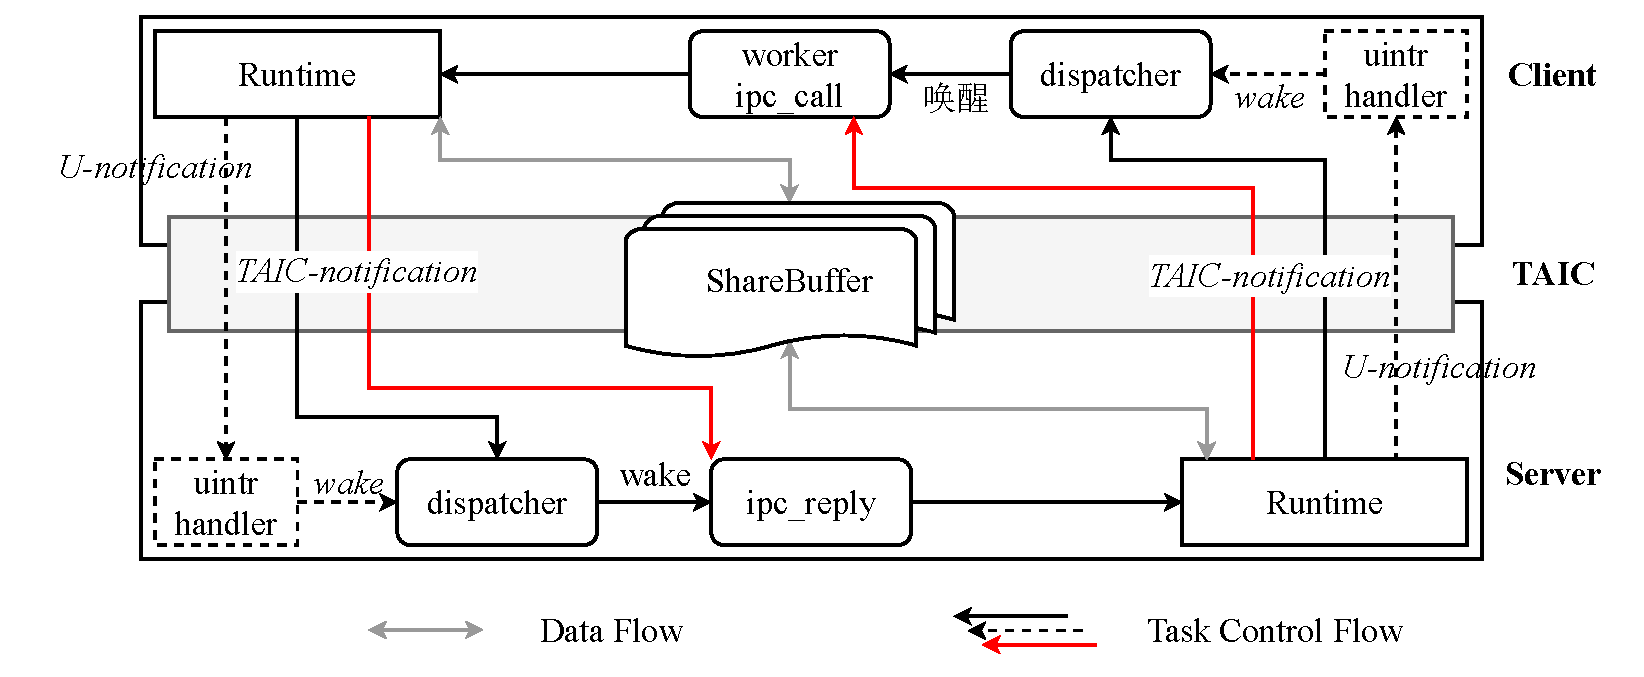
\includegraphics[width=0.9\textwidth]{figures/async_ipc.drawio.pdf}
    \caption{调度器的结构图}\label{fig:async_ipc}
  \end{figure*}

Call的主要流程分为以下几个阶段:
\begin{enumerate}
    \item 客户端发起请求:用户态程序将以worker协程的形式发起IPC请求,异步运行时首先会根据请求的数据和协程的协程号生成 IPCItem 并写入请求的环形缓冲区中并将当前协程阻塞,然后检查缓冲区的 $req\_handler\_status$ 标志位,如果对方的dispatcher协程已经就绪,那客户端无需通知对方进程,对方进程的异步运行时会在某个时刻调度到dispatcher协程并处理请求。如果对方的dispatcher协程处于阻塞状态,则异步运行时会将$req\_handler\_status$ 标志位置位,并发送U-notification通知对方进程唤醒 dispatcher协程并重启调度。
    \item 服务端处理请求并写回响应:服务端的dispatcher协程会在合适的时机读取出请求并进行解码和处理,然后根据处理结果构造响应的 IPCItem 并写入响应的环形缓冲区中,检查缓冲区中的 $req\_handler\_status$  标志位,如果客户端的响应 dispatcher协程就绪,则无需发起通知,否则需要发起U-notification通知客户端进程唤醒 dispatcher协程并重启调度。如果缓冲区内容为空,dispatcher协程会将 $req\_handler\_status$  标志位置空,并将自己阻塞。
    \item 客户端处理响应:客户端的 dispatcher协程会在合适的时机读取响应并唤醒之前阻塞的协程,然后重启调度。
\end{enumerate}

其伪代码如\ref{alg:async_ipc}所示。

\begin{algorithm}[H]
    \caption{异步IPC流程的伪代码}\label{alg:async_ipc}
    \SetKwFunction{Fn}{fn}
    \SetKwProg{Prog}{}{}{}
    \SetKw{KwAwait}{await}
    \SetKw{KwYield}{yield\_now}
    \SetKw{KwLet}{let}
    \SetKw{KwSome}{Some}
    \SetKw{KwErr}{Err}
    \SetKw{KwReturn}{return}
    
    \Prog{\Fn{async ipc\_call(cap, msg\_info) $\rightarrow$ Result<IPCItem>}}{
        item = IPCItem::new(current\_cid(), msg\_info)\;
        buffer = get\_buffer\_from\_cap(cap)\;
        buffer.req\_ring\_buffer.write(item)\;
        \If{buffer.req\_co\_status == false}{
            \tcp{设置标志位并通知对端}
            buffer.req\_co\_status = true\;
            u\_notification\_signal(cap)\;
        }
        \If{\KwLet \KwSome(reply) = \KwYield().\KwAwait}{
            \KwReturn \KwSome(reply)\;
        }
        \KwReturn \KwErr(())\;
    }
    
    \Prog{\Fn{async ipc\_recv\_reply(cap)}}{
        buffer = get\_buffer\_from\_cap(cap)\;
        \While{true}{
            \If{\KwLet \KwSome(item) = buffer.req\_ring\_buffer.get()}{
                reply = handle\_item(item)\;
                buffer.resp\_ring\_buffer.write(reply)\;
                \If{buffer.reply\_co\_status == false}{
                    buffer.reply\_co\_status = true\;
                    u\_notification\_signal(cap)\;
                }
            }\Else{
                buffer.req\_co\_status = false\;
                \KwYield().\KwAwait\;
            }
        }
    }
\end{algorithm}



\section{异步系统调用}
从广义的角度来看,异步系统调用是一类特殊的异步IPC,其接收方为内核。因此ReL4在内核中提供了一套相似的异步运行时以支持异步系统调用。异步系统调用与异步IPC的主要不同之处有两点:1) 由于接收端是内核,发送端无法使用U-notification去通知内核。2) 异步IPC中进程的异步调度器就是进程的执行主体,无需考虑异步任务的执行时机,而内核除了异步系统调用请求需要调度器执行,本身就有如中断、异常、任务调度等其他任务需要被执行。对于第一点,ReL4新增一个系统调用去用于唤醒相关的内核协程即可。而对于第二点,一个很简单的思路是每次时钟中断到来时去执行异步系统调用,然而这可能会导致空闲的CPU核心无法及时触发时钟中断而空转,因此,在不破坏原本的线程优先级调度前提下,ReL4使用核间中断来抢占空闲CPU核心或正在运行低优先级线程的CPU核心,更好地利用空闲CPU资源,减少响应时延。

为了避免破坏微内核中原本的优先级调度机制,ReL4在内核中对每个CPU核心维护了相应的执行优先级($exec\_prio$),执行优先级区别于上文提到的运行时协程优先级,是由内核调度器维护的线程优先级。内核中的任务主要分为三类:
\begin{enumerate}
  \item idle thread: 空闲CPU核心执行idle线程,此时CPU核心的执行优先级为256,属于最低的执行优先级。
  \item 内核态任务:正在处理中断、异常、系统调用等,此时CPU核心的执行优先级为0,最高优先级,不可被抢占。
  \item 用户态任务:正在执行用户态的任务,此时CPU核心的执行优先级为当前线程的优先级,可以被更高优先级线程提交的异步系统调用请求打断。
\end{enumerate}


当发送端通过系统调用陷入内核去唤醒相应协程后,会检查当前线程的优先级是否可以抢占其他CPU核心,如果可以,则发送核间中断抢占该CPU核心去执行异步系统调用,当前CPU核心则返回用户态继续执行其他协程。如果没有可以被抢占的CPU核心,则在下一次时钟中断到来时执行异步系统调用请求,其伪代码\ref{alg:wake_syscall_handler}所示:

\lstdefinelanguage{rust}{
    keywords={fn, if, let, Some, as, in},
    keywordstyle=\color{blue}\bfseries,
    ndkeywords={self, current, cid, cpu_id, exec_prio, mask},
    ndkeywordstyle=\color{magenta}\bfseries,
    identifierstyle=\color{black},
    sensitive=false,
    comment=[l]{//},
    morecomment=[s]{/*}{*/},
    commentstyle=\color{gray}\ttfamily,
    stringstyle=\color{red}\ttfamily,
    morestring=[b]',
    morestring=[b]"
}

\begin{algorithm}[H]
    \caption{唤醒内核中异步处理协程的伪代码}\label{alg:wake_syscall_handler}
    \SetKwFunction{Fn}{fn}
    \SetKwProg{Prog}{}{}{}
    \Prog{\Fn{wake\_syscall\_handler()}}{
        current = get\_current\_thread(); \\
        \If{let Some(cid) = current.async\_sys\_handler\_cid} {
            coroutine\_wake(cid); \\
            current\_exec\_prio = current.tcb\_prio; \\
            (cpu\_id, exec\_prio) = get\_max\_exec\_prio(); \\
            \If{current\_exec\_prio < exec\_prio} {
                // 抢占低执行优先级的核心 \\
                mask = 1 $\ll$ cpu\_id; \\
                ipi\_send\_mask(mask, ASYNC\_SYSCALL\_HANDLE, mask); \\
            }
        }
    }
\end{algorithm}